\documentclass[12pt,twoside]{article}

% La extensión total de la memoria deberá ser de un máximo de 50 páginas (excluidos resumen, índice y posibles anexos).

% Según las recomendaciones de estilo, el formato de la memoria se ajustará a lo siguiente:
% ? Formato del papel: DIN A4.
% ? Impresión a dos caras.
% ? Márgenes: superior e inferior, 2.5 cm. Márgenes laterales: páginas impares, izquierdo 4 cm y derecho 2 cm; páginas % pares, izquierdo 2 cm y derecho 4 cm.
% ? Tipo de letra: Times New Roman de 12 puntos.
% ? Interlineado: 1.5 líneas.
% ? Alineación: justificación completa.
% ? Sangrado de párrafo: 0.5 cm la primera línea de cada párrafo. No se
%pondrá espacio entre párrafos.
% ? Las páginas deberán ir numeradas en números arábigos.

% Teniendo en cuenta las indicaciones previas, definimos el estilo en LaTeX:

% Indicaciones para el idioma:
\usepackage[T1]{fontenc}
\usepackage[utf8]{inputenc}
\usepackage[spanish]{babel}
\usepackage{float}

% Adaptación de itemize y enumerate a los usos tipograficos españoles:
\let\layoutspanish\relax
\addto\captionsspanish{\def\tablename{Tabla}} % para que escriba "Tabla" en lugar de "Cuadro"
\unaccentedoperators  % para que no acentúe los operadores

% Área de impresión de una página:
\usepackage[a4paper]{geometry}
  \geometry{hmargin={2.5cm,2.5cm},height=22cm}

% Formato de algunas distancias:
\renewcommand{\baselinestretch}{1.2}    % separación entre líneas de un mismo párrafo
\setlength{\partopsep}{0pt}
\setlength{\itemsep}{0pt}
\setlength{\topsep}{0pt}
\setlength{\parsep}{0pt}
\setlength{\parskip}{0.25\baselineskip}   % separación entre párrafos

\renewcommand{\textfraction}{0.1}   % mínima fracción de la página para el texto
\renewcommand{\topfraction}{1}      % máxima fracción de la página para objetos flotantes en la parte superior
\renewcommand{\bottomfraction}{1}
\renewcommand{\floatpagefraction}{1}

\setcounter{totalnumber}{5}
\setcounter{topnumber}{3}
\setcounter{bottomnumber}{2}

% Adaptación de las "caption" de los entorns "figure" y "table":
\usepackage{caption}
\setcaptionwidth{\textwidth}
\addtolength{\captionwidth}{-2\parindent}
\captionsetup{margin=\leftmargini,%
  width=\captionwidth,%
  labelfont={up,bf},%
  font={small,sl},%
  %indention={\captionindent
}

% Indentación del primer párrafo de una sección:
\usepackage{indentfirst}

% Definición del color grisclaro en la salida PDF:
\usepackage[pdftex]{color}

% Gráficos:
\usepackage[pdftex]{graphicx}

% Paquetes recomendados para la inclusión de fórmulas matemáticas:
\usepackage{amsmath}
\allowdisplaybreaks  % para que pueda partir fórmulas que ocupan más de una línea, necesita el paquete anterior
\usepackage{amssymb} % para cargar algunos símbolos como \blacksquare y \square
\usepackage{amsfonts} % para cargar algunas fuentes en estilo matemático
\usepackage{enumerate}
% Teoremas (se pueden definir todos los que se necesiten):

\newtheorem{theorem}{Teorema}[section]
\newtheorem{proposition}[theorem]{Proposición}
\newtheorem{definition}[theorem]{Definición}
\newtheorem{lemma}[theorem]{Lema}
\newtheorem{corollary}[theorem]{Corolario}
\newtheorem{example}[theorem]{Ejemplo}
\newtheorem{app}[theorem]{Aplicación}
\newtheorem{remark}[theorem]{Observación}
\newtheorem{agrad}[theorem]{Agradecimiento}
\newtheorem{algo}[theorem]{Algoritmo}
\newtheorem{axiom}[theorem]{Axioma}
\newtheorem{case}[theorem]{Caso}
\newtheorem{conclu}[theorem]{Conclusión}
\newtheorem{conjectura}[theorem]{Conjetura}
\newtheorem{notac}[theorem]{Notación}
\newtheorem{soluc}[theorem]{Solución}
\newtheorem{summary}[theorem]{Sumario}


\newtheorem{proof}[theorem]{Demostración.}
\renewenvironment{proof}{\emph{Demostración.}} {\quad \hfill $\blacksquare$ \newline} % para que aparezca un cuadrado negro al acabar la demostración


% Definición de cabeceras y pies de página:

\usepackage{fancyhdr}                     % para definir distintos tipos de cabeceras y pies de página

\newcommand{\RunningAuthor}{Jose Joaquín Rodríguez García y Araceli Teruel Domenech}
\newcommand{\Author}[1]{\renewcommand{\RunningAuthor}{#1}}
\renewcommand{\leftmark}{\RunningAuthor}

\newcommand{\RunningTitle}{Trabajo de Python}
\newcommand{\Title}[1]{\renewcommand{\RunningTitle}{#1}}
\renewcommand{\rightmark}{\RunningTitle}

\pagestyle{fancy}
\fancyhf{}
\fancyhead[LO]{\small \slshape \leftmark}    % lo que aparece en la parte izquierda de la páginas impares
\fancyhead[RE]{\small \slshape \rightmark}   % lo que aparece en la parte derecha de las páginas pares
\fancyhead[RO,LE]{\small \slshape \thepage}  % el número de página aparece en la parte exterior de la cabecera

\renewcommand{\headrulewidth}{0.6pt}         % grueso de la línea horizontal por debajo de la cabecera de la página
\renewcommand{\footrulewidth}{0pt}           % grueso de la línea horizontal por encima del pie de página
                                             % en este caso está vacío
\setlength{\headheight}{1.5\headheight}      % aumenta la altura de la cabecera en una parte y media

\fancypagestyle{plain}{%                     % redefinición del estilo de página 'plain'
  \fancyhf{}                                 % limpia todas las cabeceras y pies de página
  \setlength{\headwidth}{\textwidth}
  \fancyfoot[C]{\small \slshape \thepage}    % excepto el centro del pie de página
  \renewcommand{\headrulewidth}{0pt}
  \renewcommand{\footrulewidth}{0pt}
  }

% Instrucciones que se usan frecuentemente
\newcommand{\abs}[1]{\ensuremath{|#1|}}

% Datos del trabajo y autor:
\title{Trabajo en \textit{Python}}
\author{Jose Joaquín Rodríguez García y Araceli Teruel Domenech\\*[1em]
\begin{minipage}{0.75\textwidth}
\footnotesize \itshape
\begin{center}
Universidad Politécnica de Valencia \\
Master en Big Data Analytics
\end{center}
\end{minipage}
}
\date{Septiembre 2017}

% Para incluir paginas de otro pdf (por ejemplo, la de la portada):
\usepackage{pdfpages}














\begin{document}

\maketitle
% Para introducir la portada en castellano, se guardar anexo-1-portada-memoria-tfg-matematicas.pdf en el mismo directorio:
%\includepdf[pages=1]{portada.pdf}


% Después de la portada, se introducirá un resumen del Trabajo Fin de Grado (máximo 500 palabras) en una de las lenguas oficiales y en inglés, junto con las palabras clave (de 3 a 5).

\section{Primera tarea}

Comparación de los tiempos de ejecución entre código puro de \textit{Python} y código usando la librería \textit{Numpy}.

\subsection{Primer apartado}

\subsubsection{Enunciado}

\noindent
Ordenar una lista:

\begin{enumerate}[(a)]

\item Usando bucles de \textit{Python}.

\item Usando un bucle de \textit{Python} y la función \textit{argmin} de la librería \textit{Numpy}.

\item Usando la función de ordenación de la librería \textit{Numpy}.

\end{enumerate}

\subsubsection{Resolución}

\begin{figure}[hbt]
\begin{center}
	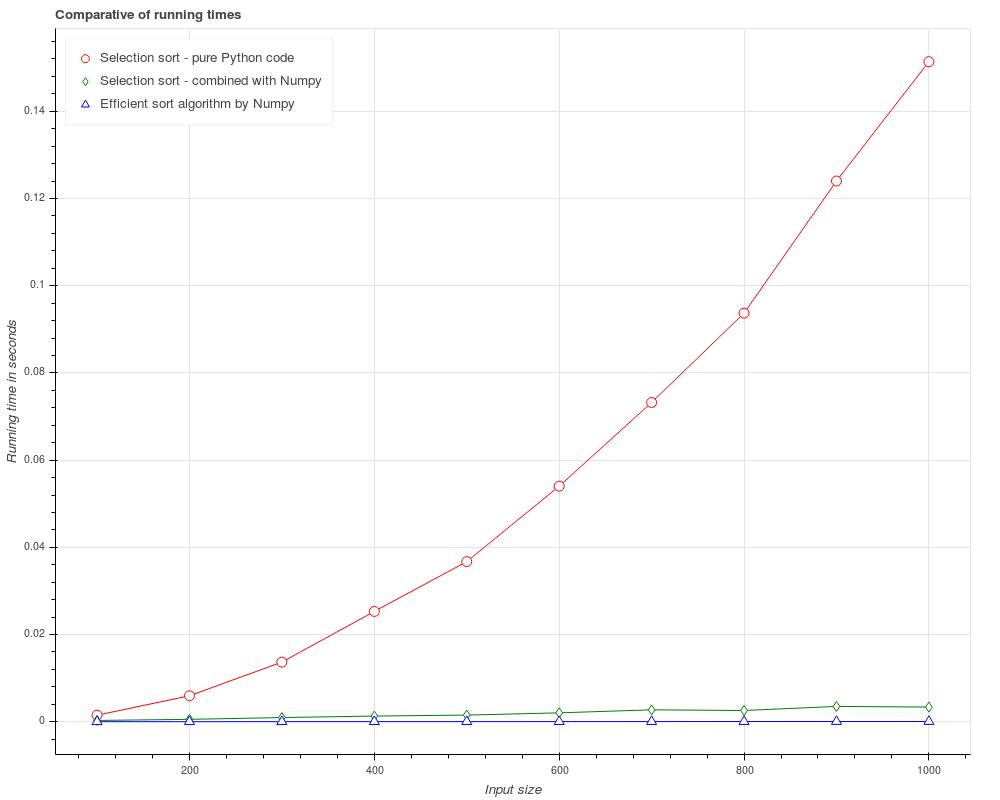
\includegraphics[width=1\textwidth]{11.png}
	\caption{Comparativa de los tiempos de ejecución de los tres scripts.}
	\label{fig:fig1}
\end{center}
\end{figure}

%Para el caso de tener que ordenar un vector de 100 elementos vemos en la figura \ref{fig:fig1} que el script más eficiente en tiempo de ejecución es el que hace uso de bucles de \textit{\textit{\textit{Python}}} junto la función argmin de la librería \textit{Numpy}. El siguiente  script más eficiente es el script que hace uso solamente de bucles de \textit{\textit{\textit{Python}}} y por último lo es el script que proporciona la librería \textit{Numpy} como función.

Usando vectores de un número mayor o igual a 100 elementos, se ve en la figura \ref{fig:fig1} que el \textit{script} más eficiente en tiempo de ejecución es el que proporciona la librería \textit{Numpy} como función, seguido del \textit{script} que usa bucles de \textit{\textit{\textit{Python}}} y la función argmin de la librería \textit{Numpy} y por último lo es el \textit{script} que usa solamente bucles de \textit{\textit{\textit{Python}}}.

Por último, comentar que al aumentar el número de elementos de un vector a ordenar, por encima de 200, el \textit{script} que hace uso de bucles de \textit{Python} ve incrementado el tiempo que necesita para la tarea de forma exponencial. Lo cual refleja que este algoritmo es muy ineficiente en términos de tiempos de computo, para ordenar una gran cantidad de elementos.
 
%Por tanto, como conclusión, si necesitamos ordenar un número reducido de elementos lo ideal es usar el \textit{script} que combina bucles de \textit{Python} con la función argmin de la librería \textit{Numpy}, mientras que si necesitamos ordenar una gran cantidad de elementos lo idoneo es usar la función que proporciona la librería \textit{Numpy} y por supuesto evitar usar solamente bucles de \textit{Python}.

\subsection{Segundo apartado}

\subsubsection{Enunciado}

\noindent
Producto escalar entre dos vectores:

\begin{enumerate}[(a)]

\item Usando listas y bucles de \textit{Python}.

\item Usando bucles de \textit{Python} y vectores de la librería \textit{Numpy}.

\item Usando el producto matricial de \textit{Python} y vectores de la librería \textit{Numpy}.

\end{enumerate}

\subsubsection{Resolución}

\begin{figure}[hbt]
\begin{center}
	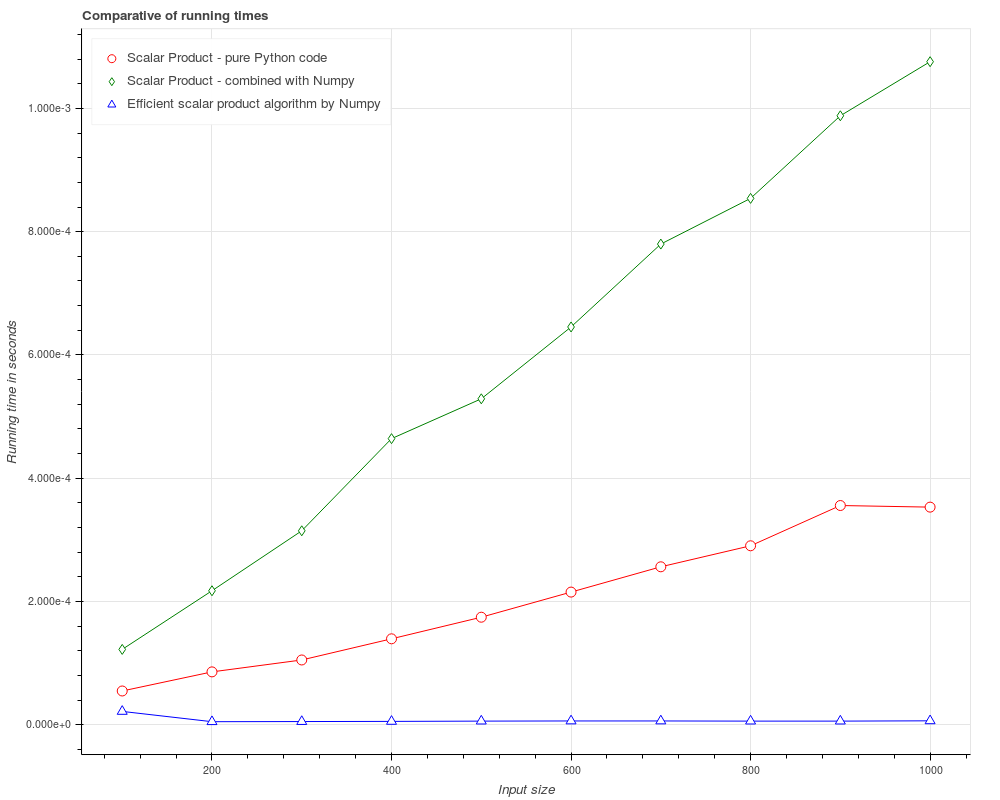
\includegraphics[width=1\textwidth]{21.png}
	\caption{Comparativa de los tiempos de ejecución de los tres \textit{scripts}.}
	\label{fig:fig2}
\end{center}
\end{figure}

Para el producto escalar de vectores con un número mayor o igual a 100 elementos vemos en la figura \ref{fig:fig2} que el \textit{script} más eficiente en tiempo de ejecución es el que hace uso del tipo de vector de la librería \textit{Numpy} combinado con la operación de producto matricial implementado en dicha librería, el siguiente más eficiente el \textit{script} que hace uso del vector como una lista de \textit{Python} y usa un bucle para recorrer los elementos de las listas y por último el menos eficiente es el que hace uso del vector como tipo de vector de la librería \textit{Numpy} y usa un bucle for para recorrer los elementos de estos vectores.

\begin{figure}[hbt]
\begin{center}
	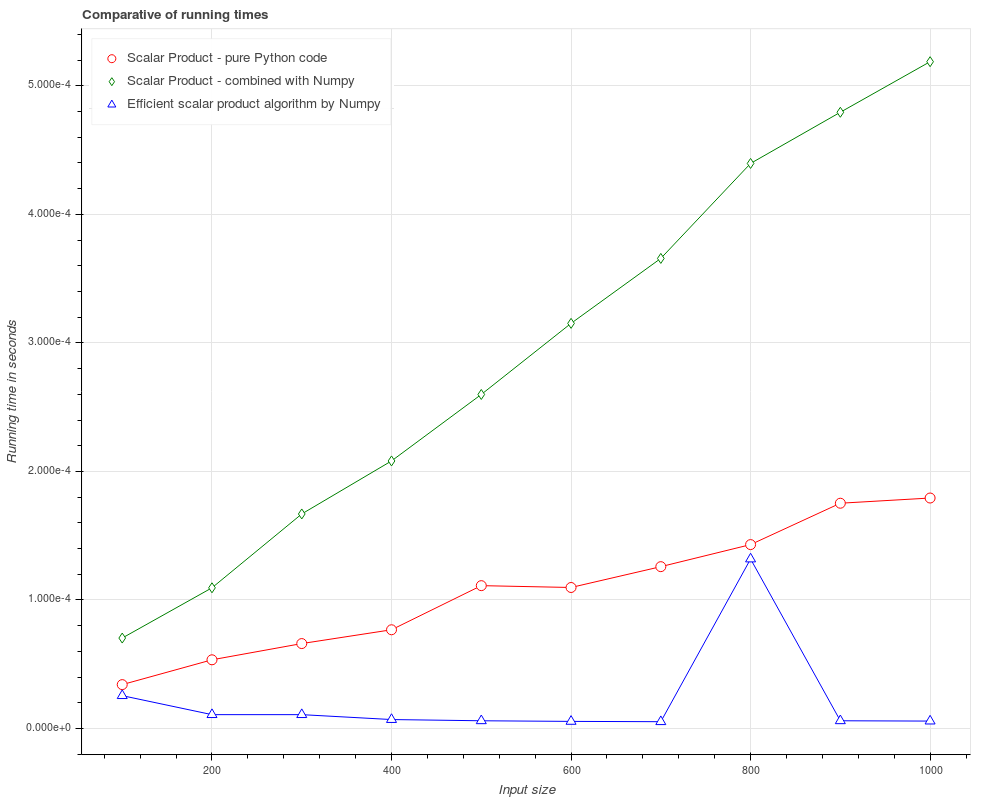
\includegraphics[width=1\textwidth]{22.png}
	\caption{Pico en el tiempo de ejecución del \textit{script} (c).}
	\label{fig:fig3}
\end{center}
\end{figure}

Se observa que el aumento del tiempo necesario para realizar el producto escalar, a medida que se aumenta el número de elementos de los vectores, tanto con el \textit{script} que usa código puro de \textit{Python} combinado con \textit{Numpy}, como con el \textit{script} que usa código puro de \textit{Python} sigue una tendencia lineal, con la diferencia de que la pendiente del primero de los \textit{scripts} comentados es más pronunciada que la del segundo \textit{script}. Mientras que el \textit{script} que usa sólo código \textit{Python} se mantiene más o menos\footnote{Haciendo varias pruebas en algunos casos se ven picos aislados, veasé por ejemplo la figura \ref{fig:fig3}, aunque estos picos siguen estando por debajo del tiempo que requieren los otros dos \textit{scripts} para llevar a cabo la operación.} constante rozando el tiempo de cómputo 0.


\subsection{Tercer apartado}

\subsubsection{Enunciado}

\noindent
Producto matricial entre un vector y una matriz:

\begin{enumerate}[(a)]

\item Usando listas y bucles de \textit{Python}.

\item Usando bucles de \textit{Python} con vectores y matrices de la librería \textit{Numpy}.

\item Usando el producto matricial de \textit{Python} con vectores y matrices de la librería \textit{Numpy}.

\end{enumerate}

\subsubsection{Resolución}

\begin{figure}[hbt]
\begin{center}
	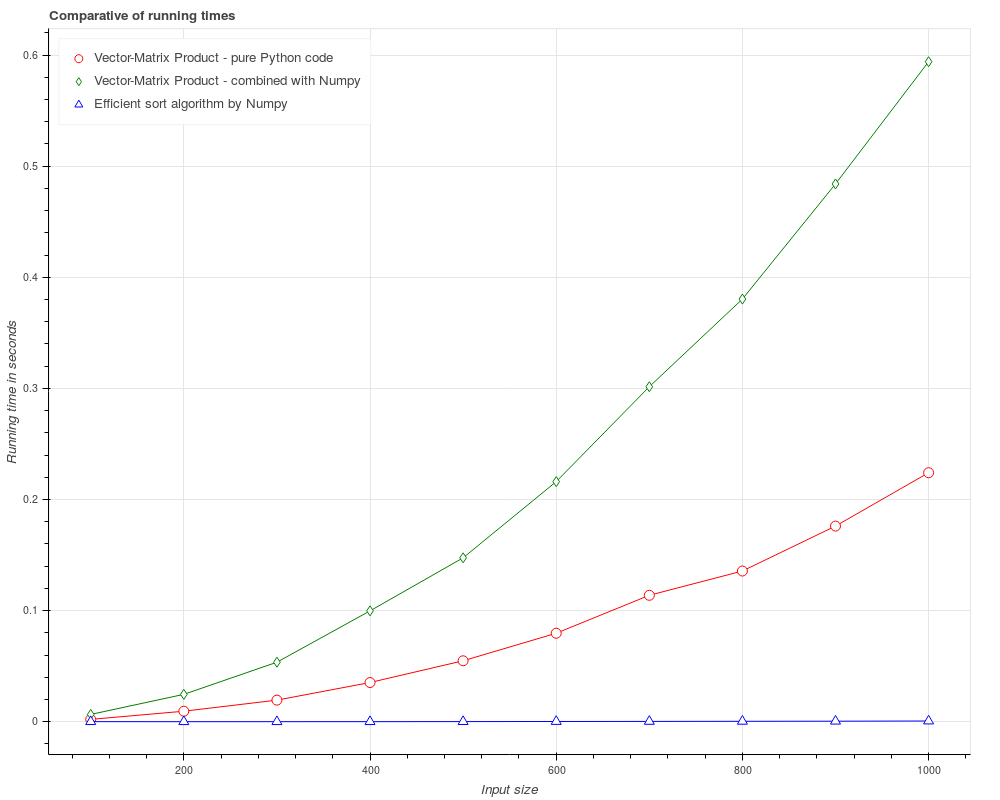
\includegraphics[width=1\textwidth]{31.png}
	\caption{Comparativa de los tiempos de ejecución de los tres \textit{scripts}.}
	\label{fig:fig4}
\end{center}
\end{figure}

Para el producto matricial de una matriz por un vector o viceversa tomando el numero $n$ de elementos del vector como 100 o más y las dimensiones de la matriz como $n \times n$, vemos en la figura \ref{fig:fig4} que el \textit{script} más eficiente en tiempo de ejecución es el que hace uso del tipo de vector de la librería \textit{Numpy} combinado con la operación de su mismo producto matricial, el siguiente más eficiente el \textit{script} que hace uso del vector y matriz como listas de \textit{Python} y usa un bucle para recorrer los elementos de las listas y por último el menos eficiente es el que hace uso del vector y matriz como tipo de vector o matriz (arrays) de la librería \textit{Numpy} y usa un bucle for para recorrer los elementos de estos vectores.

Se observa que el aumento del tiempo necesario para realizar el producto escalar, a medida que se aumenta el valor $n$ de elementos del vector y dimensiones de la matriz $n \times n$, tanto con el \textit{script} que usa código \textit{Python} combinado con la librería \textit{Numpy}, como con el \textit{script} que usa código puro de \textit{Python}, sigue un tendencia exponencial, con la diferencia de que la base del exponente de la tendencia del primero de los \textit{scripts} comentados es mayor que la base del exponente de la tendencia del segundo, siendo la tendencia del segundo \textit{script} comentado casi lineal. Mientras que el \textit{script} que usa simplemente código de la librería de \textit{Numpy} se mantiene constante rozando el tiempo de cómputo 0.

\subsection{Cuarto apartado}

\subsubsection{Enunciado}

\noindent
Producto matricial entre un vector y una matriz:

\begin{enumerate}[(a)]

\item Usando listas y bucles de \textit{Python}.

\item Usando bucles de \textit{Python} y matrices de la librería \textit{Numpy}.

\item Usando el producto matricial de \textit{Python} y matrices de la librería \textit{Numpy}.

\end{enumerate}

\subsubsection{Resolución}

\begin{figure}[hbt]
\begin{center}
	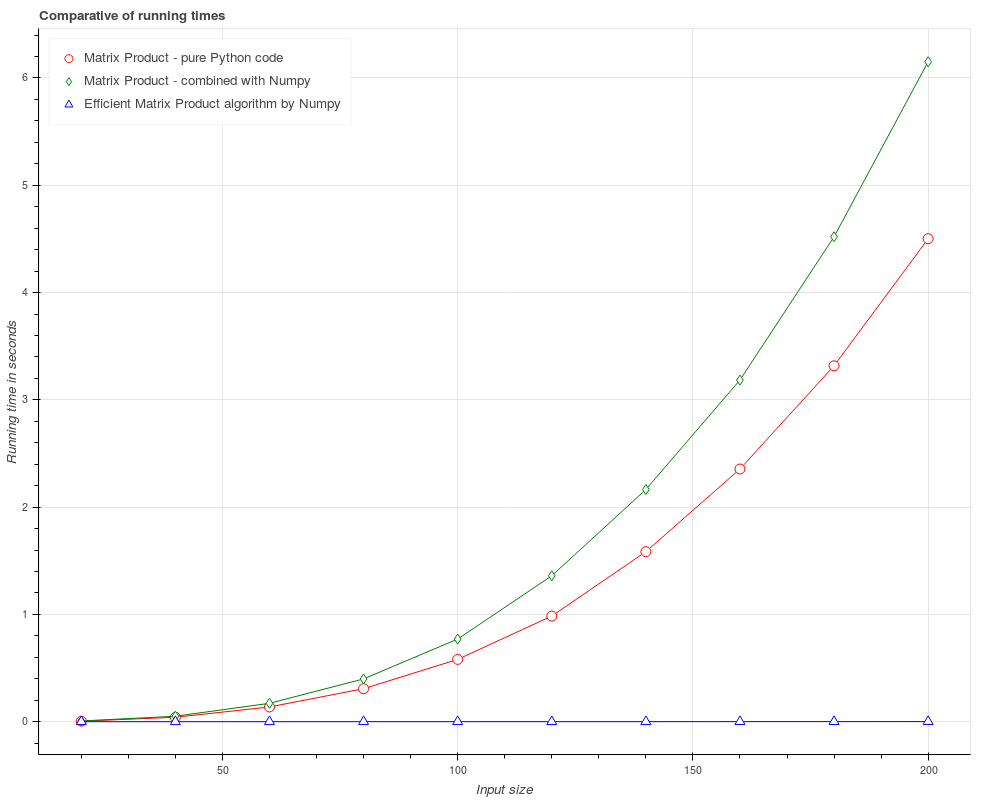
\includegraphics[width=1\textwidth]{41.png}
	\caption{Comparativa de los tiempos de ejecución de los tres \textit{scripts}.}
	\label{fig:fig5}
\end{center}
\end{figure}

Para el producto matricial de dos matrices cuadradas $n \times n$, siendo $n$ mayor o igual a 100, vemos en la figura \ref{fig:fig5} que el \textit{script} más eficiente en tiempo de ejecución es el que hace uso del tipo de matriz de la librería \textit{Numpy} combinado con la operación de producto matricial de esta misma librería, el siguiente más eficiente es el \textit{script} que trata a ambas matrices como listas de \textit{Python} y usa un bucle para recorrer los elementos de las listas y por último el menos eficiente es el que hace uso de ambas matrices como tipo de matrices de la librería \textit{Numpy} y usa un bucle for para recorrer los elementos de estas matrices. En la Figura \ref{fig:fig6} podemos ver, que esto sigue siendo así aunque el tamaño del vector sea pequeño, aunque, al contrario que en los otros casos, la diferencia es bastante menor.

%\begin{figure}[hbt]
%\begin{center}
%	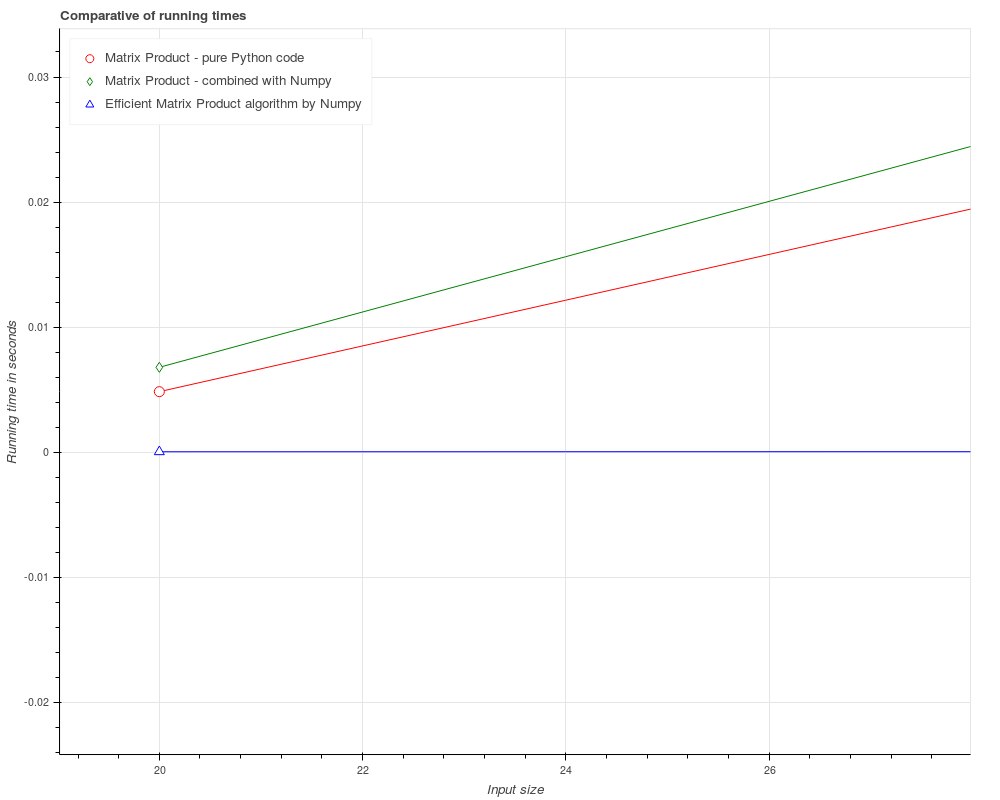
\includegraphics[width=1\textwidth]{42.png}
%	\caption{Comparativa de los tiempos de ejecución de los tres scripts.}
%	\label{fig:fig6}
%\end{center}
%\end{figure}

Se observa que el aumento del tiempo necesario para realizar el producto matricial, a medida que se aumenta el valor $n$ de las dimensiones de las matrices, tanto con el \textit{script} que combina la librería \textit{Python} con código puro, como con el \textit{script} que usa sólo código puro de \textit{Python}, sigue un tendencia exponencial, con la diferencia de que la base del exponente de la tendencia del primero de los \textit{scripts} comentados es mayor que la base del exponente de la tendencia del segundo. Mientras que el \textit{script} que usa la librería de \textit{Numpy} tanto para la definición de las matrices como para el producto de ellas se mantiene constante rozando el tiempo de cómputo 0.

\subsection{Conclusión}
Como hemos podido comprobar, siempre que usemos la librería \textit{Numpy} para todo el cálculo será mucho más eficiente en tiempo de ejecución. Pero si vamos a usar código puro de \textit{Python} para realizar algún cálculo, es más eficaz, en cuanto a tiempo de computo, el definir las variables que vayamos a usar usando la librería \textit{Numpy}, ya que la diferencia es bastante notable en todos los casos. Por último comentar que el código puro de \textit{Python} para un número reducido de elementos (un número menor o igual a $100$) no presenta diferencias significativas, cuanto a tiempo de computo, con el resto de los \textit{scripts} usados.

\section{Segunda tarea}

\subsection{Enunciado}

Escribir un código en \textit{Python} que:

\begin{enumerate}

\item Cargue la matriz A y el vector b de un archivo del disco.

\item Resolver el sistema $Ax=b$, es decir, obtener el vector $x$.

\item Mostrar los resultados por pantalla para comprobar que son realmente una solución.

\end{enumerate}

\subsection{Resolución}

Comenzamos el ejercicio llamando a la función \textit{subprocess.call} para que cada vez que ejecutemos el ejercicio, nos genere un sistema de cinco ecuaciones con cinco incógnitas.
Al ejecutarlo nos genera la \textbf{Ecuación (\ref{Eq1})}:

\begin{equation}
		\left(
			\begin{array}{ccccc}
				18  & 12 & 15 & 6 & 1 \\
				3 & 9  & 7 & 6 & 0 \\
				0  & 0 & 15 & 7  & 19 \\
				3  & 2  & 13  & 17 & 7 \\
				4 & 17 & 18  & 14  & 19 \\
			\end{array}
		\right)
		\times
		\left(
			\begin{array}{c}
				x_1 \\
				x_2 \\
				x_3 \\
				x_4 \\
				x_5 \\
			\end{array}
		\right)
		=
		\left(
			\begin{array}{c}
				575 \\
				264 \\
				411 \\
				490 \\
				754 \\
			\end{array}
		\right),
\label{Eq1}
	\end{equation}

donde la solución a dicha ecuación es \textbf{(\ref{Eq2})}:

\begin{equation}
	\left(
		\begin{array}{c}
			x_1 \\
			x_2 \\
			x_3 \\
			x_4 \\
			x_5 \\
		\end{array}
	\right)
	=
	\left(
		\begin{array}{c}
			15 \\
			9 \\
			6 \\
			16 \\
			11 \\
		\end{array}
	\right).
	\label{Eq2}
\end{equation}

Una vez tenemos cargados los datos, los convertimos a \textit{vectores n-dimensionales} de la librería de \textit{Numpy} y finalmente resolvemos la ecuación con la función \textit{numpy.linalg.solve}.
Todo este proceso es resumido en la figura \ref{fig:fig6}.

\begin{figure}[hbt]
\begin{center}
	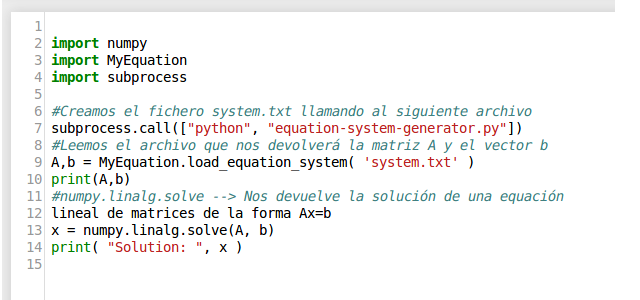
\includegraphics[width=0.9\textwidth]{task2.png}

	\caption{\textit{script} modificado con las impresiones por pantalla de los resultados obtenidos.}
	\label{fig:fig6}
\end{center}
\end{figure}


%\begin{figure}
%\begin{center}
%	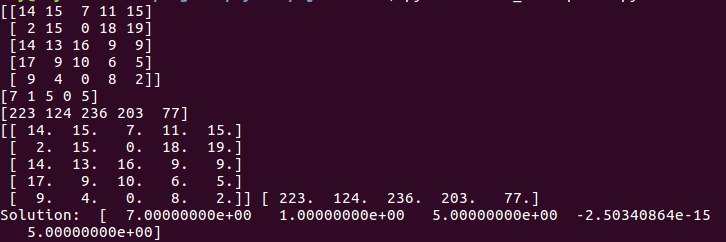
\includegraphics[width=1\textwidth]{23.png}
%	\caption{Resultados}
%	\label{fig:fig8}
%\end{center}
%\end{figure}

\end{document} 